%! Tex program = xelatex
\documentclass[UTF8]{article}
\usepackage{indentfirst}
\usepackage{graphicx} 
\usepackage{amsmath}  
\usepackage{float}   
\usepackage{listings}

\title{Discrete Mathematics}
\author{Zhengren Wang 2019081308021}
\date{06/02/2020 Tue}
\begin{document}
\maketitle 

\part{10.4}
\begin{description}
    \item[7]What do the connected components of acquaintanceship graphs represent?\\\\
        For any two people (A,B) in the same component, we can find out a set of acquaintances for us as a bridge to start walking with A and end with B.


    \item[11]Determine whether each of these graphs is strongly connected and if not, whether it is weakly connected.  \\
        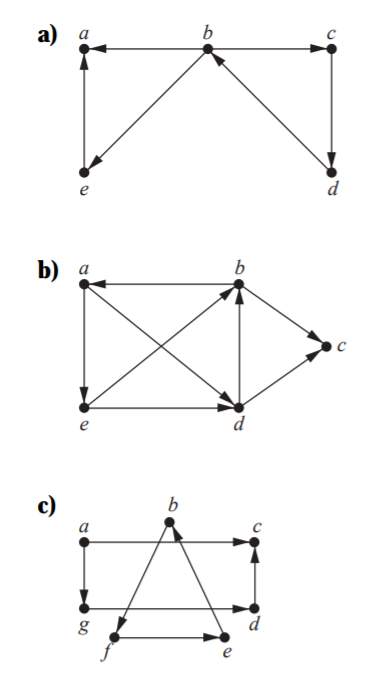
\includegraphics[scale=0.3]{../imgs/10_4_11.png}\\\\
            a) weakly connected                \\
            b) weakly connected                \\
            c) Neither of them\\


\end{description}

\end{document}
